\documentclass{article}
\usepackage{amsmath, amssymb, amsthm}
%\usepackage{newtxtext, newtxmath}
%\usepackage{newtx}
\usepackage[margin=1in]{geometry}
\usepackage{graphicx}
\usepackage[font=small,labelfont=bf]{caption}
\usepackage{subcaption}

\graphicspath{ {../images/} }

\title{Removing Projective Distortion from Images}
\author{Mickey Smith}
\date{August 2019}

\begin{document}

\maketitle

\section{Homogenous Coordinates}
Similar to cartesian coordinates, homogenous coordinates are a method to represent specific in a given dimension.

\begin{figure}[hbt!]
\centering
\begin{subfigure}{.5\textwidth}
    \centering
    \begin{pmatrix}
        x \\
        y
    \end{pmatrix}
    \caption{Cartesian $\mathbb{R}^2$}
    \label{fig:coords_sub1}
\end{subfigure}%
\begin{subfigure}{.5\textwidth}
    \centering
    \begin{pmatrix}
        x \\
        y \\
        1
    \end{pmatrix}
    \caption{Homogenous $\mathbb{R}^2$}
    \label{fig:coords_sub2}
\end{subfigure}
\caption{Representing coordinates as homogenous and cartesian}
\label{fig:coords}
\end{figure}

Note that the only practical difference between cartesian and homogenous representations (for the purposes of this assignment) is that homogenous coordinates contain an extra dimension value that represents vector scaling. This allows a point to be further from the origin on its vector passing through the origin without altering the other coordinates.

\begin{figure}[h]
    \centering
    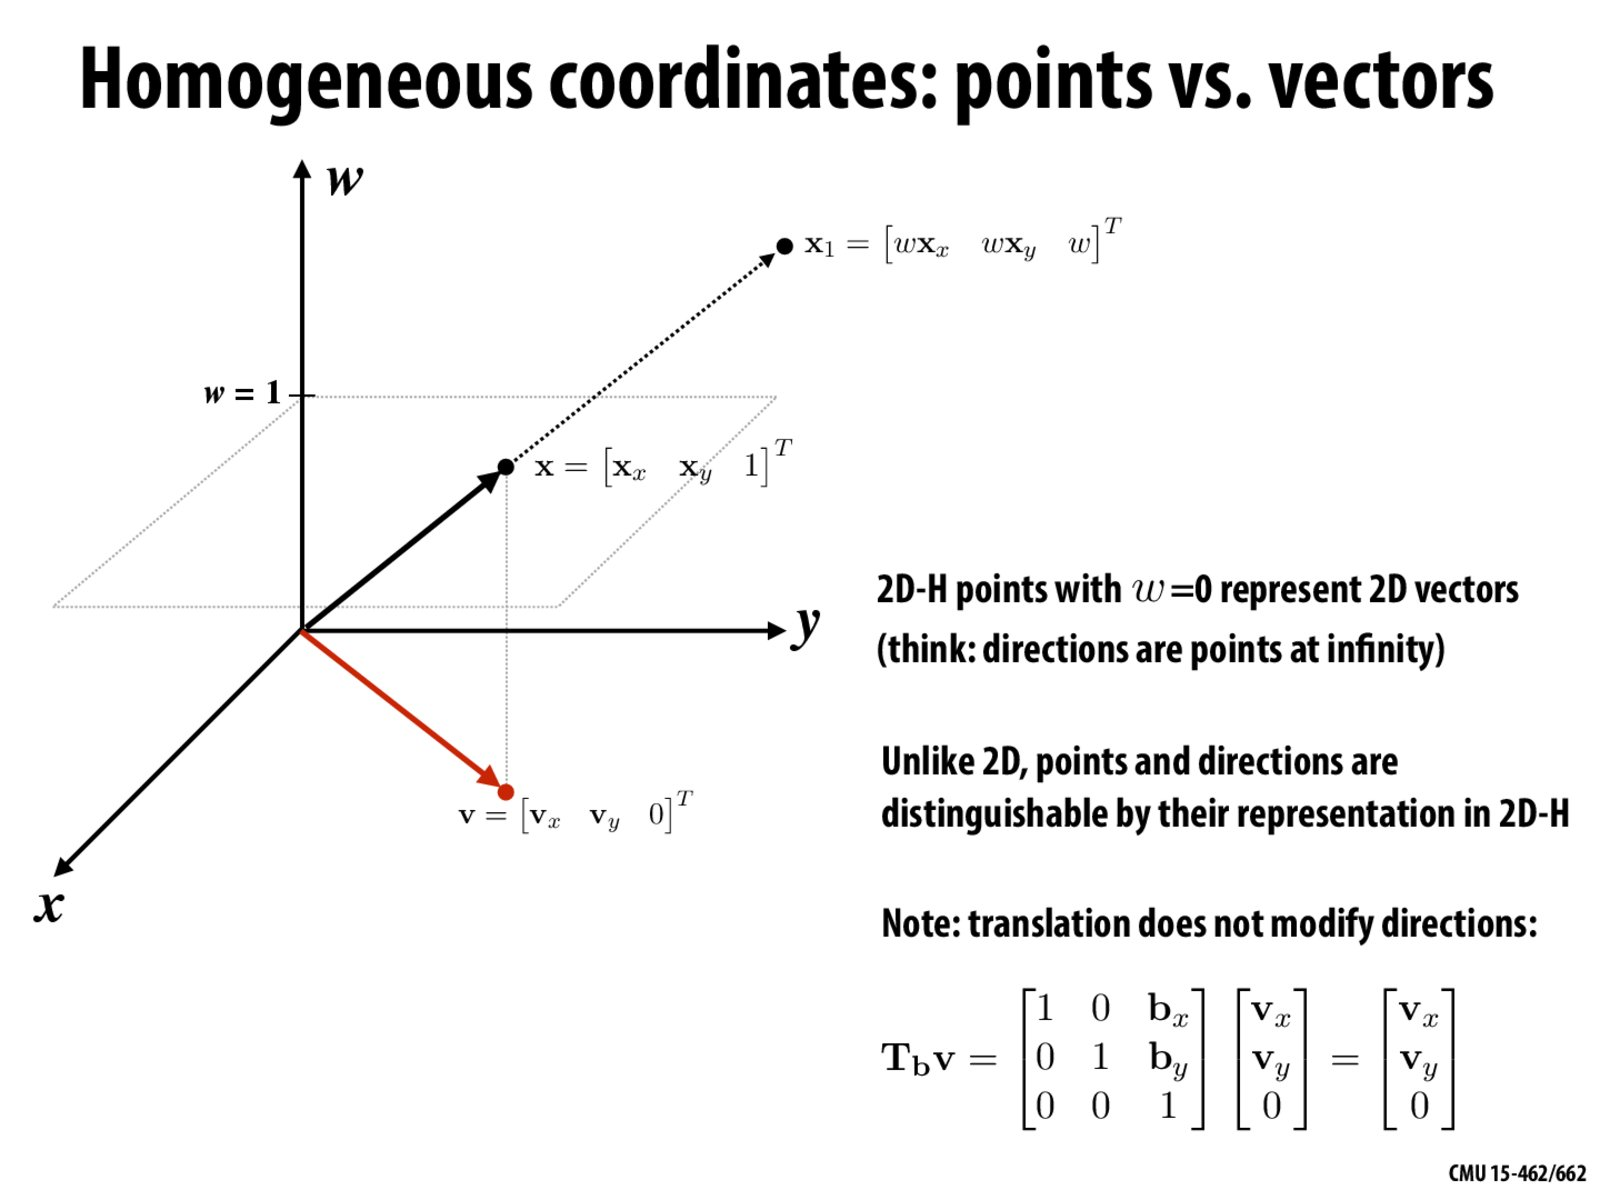
\includegraphics[scale=0.15]{homogenous_coords}
    \caption{Explanation of homogenous coordinates}
\end{figure}

\clearpage

\section{Projective Transformations}
When a photo is taken of a scene, the camera applies a transformation to the original scene in the form of a matrix called the \textit{homography}, creating a new perspective captured by the photo. An original scene \( \textbf{x} \) manipulated by a camera and resulting in a photo becomes \( \textbf{x}' \) through the application of a projective homography transformation \( H \).

\begin{figure}[h]
    \centering
    \( \textbf{x}' \) = \( H\textbf{x} \)
    \caption{Homography application. \( \textbf{x} \) represents the original scene and \( \textbf{x}' \) represents what we see in a photograph taken of the scene at an angle.}
\end{figure}

This equation is notably of the form \( Ax = B \), which will allow us to solve for the homography matrix easily\footnotemark.
\footnotetext{For the purposes of this assignment the Python library Numpy's \textit{linear algebra} class' \textit{solve()} method is used to compute the solution vector \( x \).}

In order to restore the original image's perspective we need to determine the homography matrix's inverse, \( H^{-1} \), not just the homography matrix itself. Once we have \( H^{-1} \) we can apply it to every pixel in the image to determine where it should be placed within the new image.

In order for a program to apply these inverse transformations, 8 coordinates within $\mathbb{R}^2$ have to be defined. 4 representing the corners of a box within the supplied image and 4 representing the destination location of those points within the new image that represents the real orthogonal world view of the image. We'll choose those locations as the corners of a rectangle within the image.

\begin{figure}[h]
\centering
\begin{subfigure}{.5\textwidth}
    \centering
    \begin{pmatrix}
        \( x^{ll} \) \\
        \( x^{lr} \) \\
        \( x^{ul} \) \\
        \( x^{ur} \)
    \end{pmatrix}
    \caption{Image points}
    \label{fig:coords_sub1}
\end{subfigure}%
\begin{subfigure}{.5\textwidth}
    \centering
    \begin{pmatrix}
        \( x^{'ll} \) \\
        \( x^{'lr} \) \\
        \( x^{'ul} \) \\
        \( x^{'ur} \)
    \end{pmatrix}
    \caption{World points}
    \label{fig:coords_sub2}
\end{subfigure}
\caption{User-defined parameters (where a point exists within the photograph and where it should exist in a warped view of the photograph to represent a different perspective).}
\label{fig:coords}
\end{figure}

Once these 8 points have been defined they can be placed into the \( A \) and \( B \) matrices for the \( Ax=B \) equation and used to solve for H. The ultimate equation will be an 8x8 \( A \) matrix multiplied with an 8x1 H matrix resulting in an 8x1 \( B \) matrix[Figure \ref{fig:ax_b}].

\begin{figure}[h]
    \centering
    \begin{gather}
        \begin{pmatrix}
            \( x^{i} & y^{i} & 1 & 0 & 0 & 0  & -x^{i}x^{'i} & -x^{i}y^{'i} \) \\
            \( 0 & 0 & 0 & x^{i} & y^{i} & 1 & -y^{'i}x^{i} & -y^{'i}y^{i} \)
        \end{pmatrix}
        \begin{pmatrix}
            \( h_{1} \) \\
            \( h_{2} \) \\
            \( h_{3} \) \\
            \( h_{4} \) \\
            \( h_{5} \) \\
            \( h_{6} \) \\
            \( h_{7} \) \\
            \( h_{8} \) \\
            \( h_{9} \)
        \end{pmatrix}
        =
        \begin{pmatrix}
            \( x^{'i} \) \\
            \( y^{'i} \)
        \end{pmatrix}
    \end{gather}
    \caption{Homography application}
    \label{fig:ax_b}
\end{figure}

\end{document}
